\documentclass[10pt,twocolumn,letterpaper]{article}

\usepackage{times}
\usepackage{epsfig}
\usepackage{graphicx}
\usepackage{amsmath}
\usepackage{amssymb}

% Include other packages here, before hyperref.

% If you comment hyperref and then uncomment it, you should delete
% egpaper.aux before re-running latex.  (Or just hit 'q' on the first latex
% run, let it finish, and you should be clear).
\usepackage[breaklinks=true,bookmarks=false]{hyperref}



\setcounter{page}{1}
\begin{document}


%%%%%%%%%%%%%%%%%%%%%%%%%%%%%%%%%%%%%%%%%%%%%%%%%%%%%%%%%%%%%%%
% DO NOT EDIT ANYTHING ABOVE THIS LINE
% EXCEPT IF YOU LIKE TO USE ADDITIONAL PACKAGES
%%%%%%%%%%%%%%%%%%%%%%%%%%%%%%%%%%%%%%%%%%%%%%%%%%%%%%%%%%%%%%%



%%%%%%%%% TITLE
\title{Using Machine Learning to Address the Opioid Crisis}

\author{Megan Skrobacz\\
{\tt\ skrobacz.m@northeastern.edu}
\and
Matthew Menzi\\
{\tt\ menzi.m@northeastern.edu}
\and
Yoselyn Cervantes\\
{\tt\ cervantes.y@northeastern.edu}
\and
Adithya Chundailthodi\\
{\tt\ chundailthodi.a@northeastern.edu}
}

\maketitle
%\thispagestyle{empty}



% MAIN ARTICLE GOES BELOW
%%%%%%%%%%%%%%%%%%%%%%%%%%%%%%%%%%%%%%%%%%%%%%%%%%%%%%%%%%%%%%%


%%%%%%%%% ABSTRACT
\begin{abstract}
   \textit{According to the US Center for Disease Control and Prevention, since 1999 almost 850,000 people have died from drug overdoses, and in 2019 more than 70\% of these deaths were attributed solely to opioids \cite{cdc:dataOverview}. While previous studies have used publicly-available data and machine learning models to try and aid in solving this crisis, the vast majority of previous works have focused mainly on users of opioids, specifically using models to predict an individual's chance to become addicted to opioids. For our contribution to this body of work, we instead focus on another side of the opioid supply chain: opioid prescribers. We tackle this topic on three separate fronts, narrowing our analyses to the United States. We first analyze possible influencers to opioid prescribing rates, specifically whether we can find any correlation between pro-prescription lobbying efforts and opioid prescribing rates. We then test several machine learning models to fit a predictor which can identify providers likely to be prescribers of opioids. Finally, we take that model, trained on national data, and apply it to a hyper-local dataset for the state of Connecticut to see if we can garner any additional insights. Surprisingly, we find that lobbying efforts didn't have as much of an impact as we thought on opioid distribution rates, despite the huge sums of money being used for said efforts. We also find that Gradient Boosting worked best for both our national predictor model as well as our state-level analysis.}
\end{abstract}

%%%%%%%%% BODY TEXT

%-------------------------------------------------
\section{Introduction}
%-------------------------------------------------

Opioid addiction and overdose have become tragic and inescapable threads in the fabric of American daily life. Many Americans know someone who has died of a drug overdose, and even if they do not, headlines announcing high-profile overdose deaths are common news items. Among the hundreds of thousands of opioid related deaths in the past few years are celebrated musicians Prince, Mac Miller, and Tom Petty; accomplished athletes including pitcher Tyler Skaggs, football player Jake Ehlinger, and NHL player Jimmy Hayes; and lauded actors like Philip Seymore Hoffman.

Data also sheds insight into the scope of this epidemic. According to the United States Center for Disease Control, in 2019 more than 50,000 people in the United States died from opioid-related overdoses \cite{dataabuse.gov}. It is also estimated that 3 million Americans suffer from opioid use disorder, and in 2020, a staggering 93,000 people died in the United States from drug overdoses \cite{stobbe}, most of which were related to opioids. Additionally, studies estimate that the total "economic burden" of prescription opioid misuse in the United States is \$78.5 billion a year, including the costs of healthcare, lost productivity, addiction treatment, and criminal justice involvement \cite{dataabuse.gov}. While the United States is certainly not the only country suffering from this epidemic, statistics like these make it clear that COVID-19 is not the only major medical crisis nations are struggling to contain at the moment.

Despite numerous studies related to opioid use, we feel there is ample room to take a “deep dive” into publicly-available data and see if we can draw useful conclusions to perhaps provide insight into qualming this crisis. We plan to focus US federal and state datasets to both take a broad look at the situation while also allowing us to delve deeper into more localized data to potentially find trends. More specifically, we hope to place more emphasis on examining the impact of opioid prescribers instead of focusing solely on opioid users, as has been done in other studies. To do this, will first test various machine learning models to try and create classifiers to predict the likelihood that a given doctor is a significant prescriber of opioids using a national dataset. We will then take that model and use it for analysis of a more local dataset -- specifically for the state of Connecticut -- to see if we can find relationships between prescribers who are classified as likely to prescribe opioids and the side effects of opioids, such as drug overdose and rehab data. Finally, we will look to see if other outside factors could be potentially affecting the rate of opioid prescriptions, specifically investigating if we can find a correlation between lobbying efforts of pro-drug interest groups to the amount of opioids prescribed in the region where they exert influence.

While we do have high hopes for this project, we acknowledge that we are tackling a tough issue that does not necessarily have a perfect answer which can be prescribed by a single machine learning algorithm; indeed, some data we'd like to ideally have for our analysis (such as a better insight into the prevalence of illegal opioids by geography) are simply not available. We also recognize that we have certain limitations geographically on our datasets, as our data is only focused only on the United States. However, we are confident that our exploratory analysis will shed some insights into the nature of this crisis worldwide.

%-------------------------------------------------
\section{Related Work}
%-------------------------------------------------

There have been several research efforts centered around this topic, particularly in the fields of machine learning and data science, even within the realm of individual study. For example, both Tara Boyle's "The Opioid Crisis in Data" \cite{boyle2019:online} and Kiros Gebremariam's capstone project \cite{KirosGPr71:online} use machine learning for exploratory analyses of opioid prescription trends. In both Boyle and Gebremariam's works, their analyses of publicly-available federal datasets show that of all medical specialities, general practitioners in family practice and internal medicine prescribed the greatest number of opioids. Additionally, Hydrocodone/Vicodin was far and above the most commonly-prescribed opioid, with more than double the amount of units than the second most-common opioid, Tramadol/Ultram, for the year 2016.

The majority of scholarly research is focused around predicting one's chances of opioid abuse disorder based on personal characteristics, as opposed to focusing on the prescribers themselves. Several studies, such as Huinker's analysis \cite{huinkerpaper} go into more detail about possible machine learning algorithms which can be applied to predict the possibility of opioid abuse disorder. Huinkers' study uses four popular machine learning algorithms -- Decision Trees, Artificial Neural Networks, Support Vector Machines, and Logistic Regression -- and ultimately finds a SVM with k-fold cross-validation to be the superior model for predicting individual opioid misuse. Similarly, Lo-Ciganic W et al \cite{10.1001/jamanetworkopen.2019.0968} conclude that machine learning algorithms using administrative data appear to be a valuable and feasible tool for more accurate identification of opioid overdose risk.

Despite these insights, there have been several recent works which highlight potential issues with these models. Rather than try to develop models for opioid abuse indicators, Angela Kilby \cite{10.1145/3442188.3445891} investigates issues with such algorithmic methods currently being used in locales such as medical offices and police departments. Kilby's work, which uses several proprietary datasets, finds that machine-generated risk scores are a form of algorithmic unfairness in machine learning applications as they are heavily dependent on the researcher's choice of objective function, and as such are not reliable indicators of actual risk when deciding treatment. Indeed, critique of machine learning algorithms predicting one's chances of opioid abuse is so prevalent that even mainstream journalistic sources cover the topic. For example, Szalavitz's exposé in Wired \cite{wiredarticle:online} displays how such algorithms currently in use by doctors and drug companies have unfairly discriminated against patients with complex or chronic illnesses, histories of sexual abuse, and women.

%-------------------------------------------------
\section{Proposed Method}
%-------------------------------------------------

\subsection{Lobbying Analysis}


\subsection{Prescriber Classifier Analysis}

The following classification algorithms were used to build our prediction model:

\paragraph{Perceptron.} The key idea here is to separate the input into two categories, positive or negative, by drawing a line (a linear operation) in the feature space. The algorithm iteratively corrects misclassifications by adjusting the classification line or boundary. 

We can represent the perceptron in vector form as follows:

$$h(x) = \sin\left(\sum_{i=0}^dw_ix_i\right) = \sin\left(w^Tx\right)$$

Each “tall” \emph{w} represents a hypothesis \emph{h} and is multiplied with “tall” \emph{x}.

\paragraph{KNearestNeighbors.} The key idea here is to find which training data is closest to the test instance, and classify the test instance as that class.

Majority vote from k-nearest neighbors is defined as:

$$y = argmax\sum_{\left(x_i,y_i\right)\in D_z}I\left(v = y_i\right)$$

where:
\begin{itemize}
 
   \item \emph{v} is a class label
   \item $y_i$ is the class label for one of the nearest neighbors
   \item \emph{I} is the  indicator function (i.e., 1 if the argument is true, 0 otherwise).

\end{itemize}

\paragraph{Gaussian Naïve Bayes.} The algorithm assumes that selected features are equally important and statistically independent (given the class value). 

With the independence assumption, the probability of class yj generating instance x can 
then be estimated as:

$$P\left(x\vert y_j\right)\;=\;P\left(x_1\vert y_j\right)\;\times\;P\left(x_2\vert y_j\right)\;\times\;...\;\times\;P\left(x_n\vert y_j\right)$$

\paragraph{Decision Trees.} This model follows a directed tree structure composed of nodes where each node specifies an evaluation on a feature and each branch corresponds to a feature value/condition. The leaves signify categorical decision or class. The main reasons for using decision trees are that the decision trees: 

\begin{itemize}
 
   \item Divide the feature space into axis parallel rectangles , thus providing an easy method for distinctly dividing the feature set as opioid or non opioid based on the input feature set.
   \item The target function is discrete valued and decision trees work well in predicting discrete valued target functions.

\end{itemize}

\paragraph{Gradient Booster.} Gradient boosting works by building simpler (weak) prediction models sequentially where each model tries to predict the error left over by the previous model. We combine many weak learners to come up with one strong learner. The weak learners here are the individual decision trees.

\emph{Learning rate} and \emph{n\_estimators} are two critical hyperparameters for gradient boosting decision trees. Learning rate, denoted as $\alpha$, simply means how fast the model learns. Each tree added modifies the overall model. The magnitude of the modification is controlled by learning rate. The lower the learning rate, the slower the model learns. That takes more time to train the model which brings us to the other significant hyperparameter. The n\_estimator is the number of trees used in the model. For our model, we used a learning rate of 0.1 and n\_estimator of 200. Since we are using Gradient Booster as a classifier, the cost function is Log loss.


\subsection{State-Specific Analysis}



%-------------------------------------------------
\section{Experiments}
%-------------------------------------------------

\subsection{Lobbying Analysis}


\subsection{Prescriber Classifier Analysis}

\begin{figure}[t]
   \begin{center}
      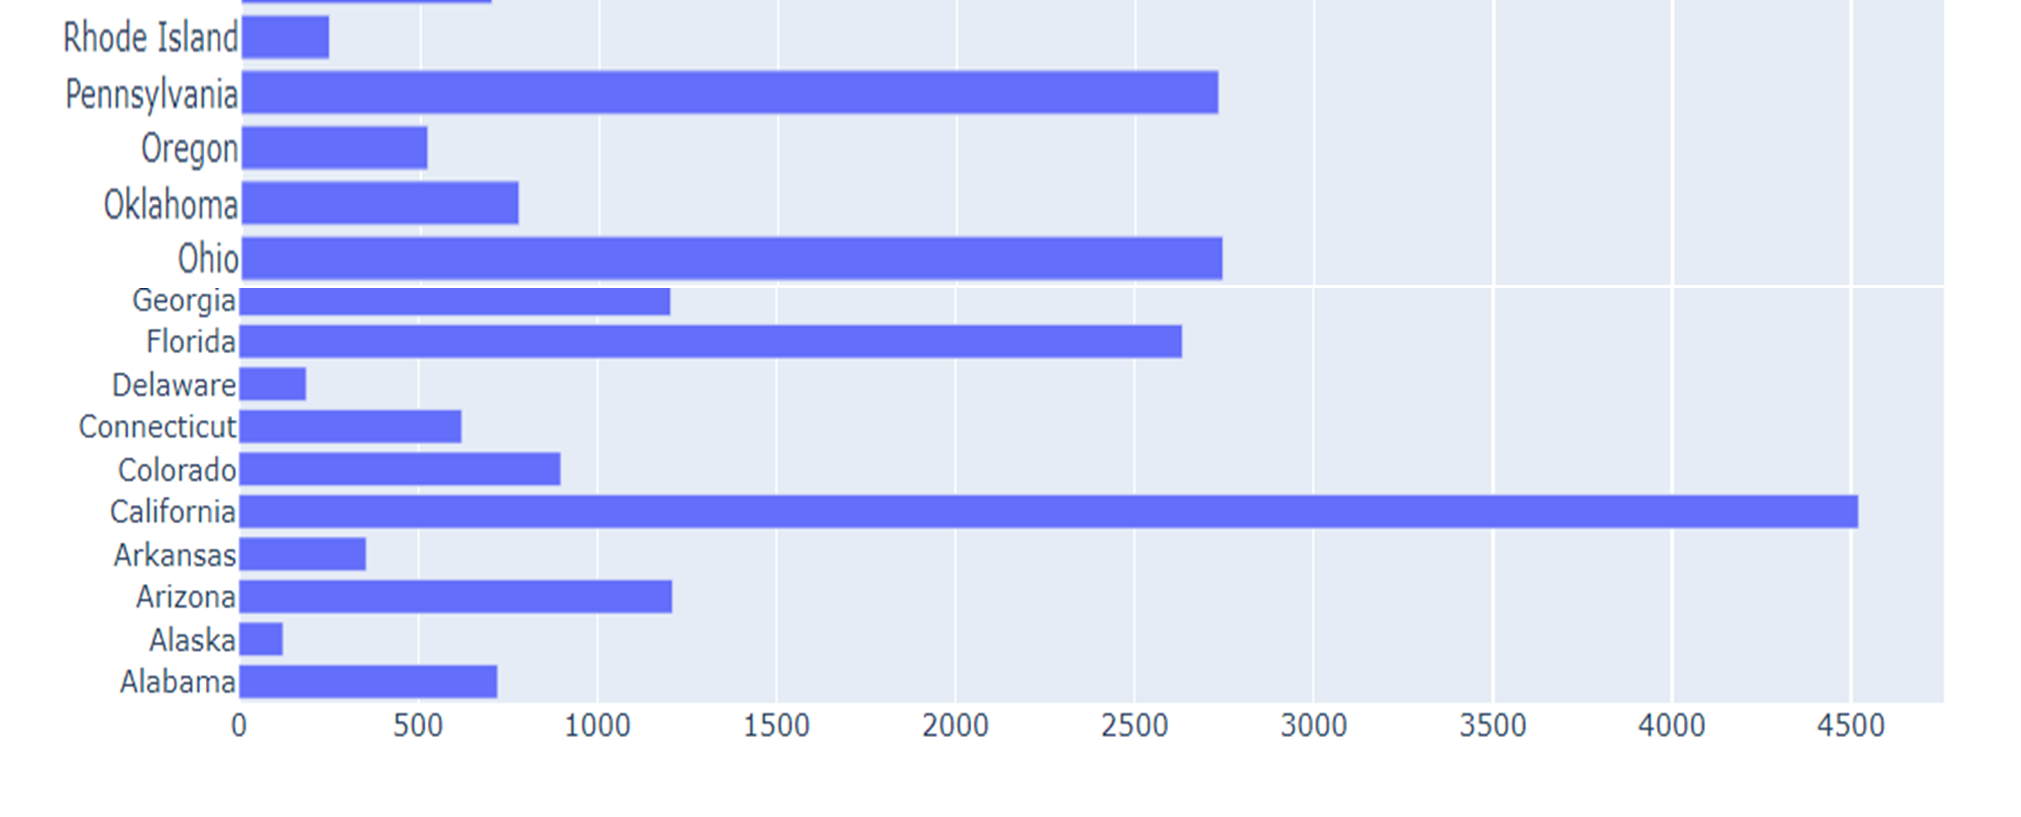
\includegraphics[width=1.0\linewidth]{figures/states1.png}
   \end{center}
      \caption{Overdose Deaths Per State}
   \label{fig:google-scholar-1col}
\end{figure}

\begin{figure}[t]
   \begin{center}
      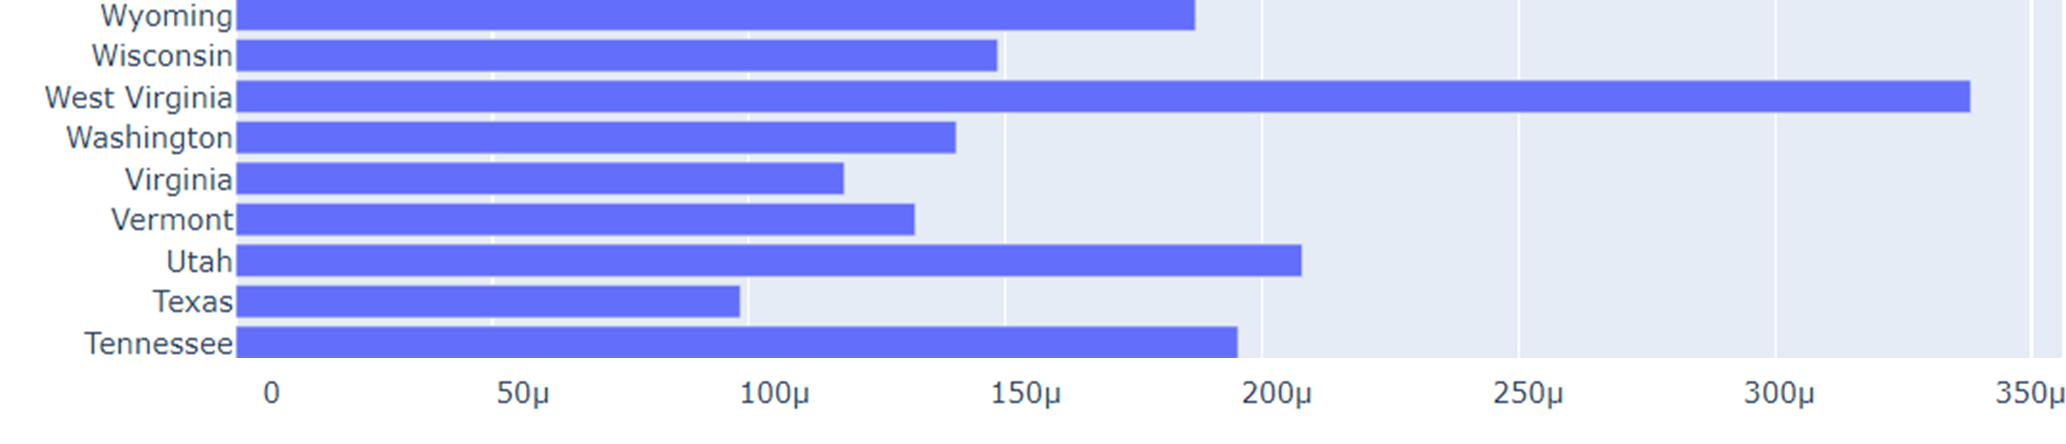
\includegraphics[width=1.0\linewidth]{figures/states2.png}
   \end{center}
      \caption{Overdose Deaths Per State and Per Capita}
   \label{fig:states2-1col}
\end{figure}

\begin{figure}[t]
   \begin{center}
      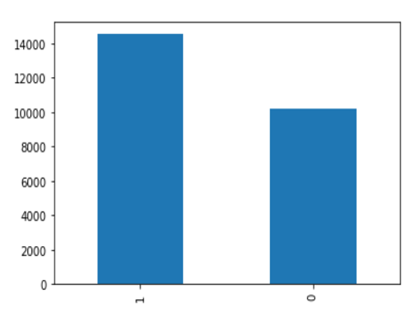
\includegraphics[width=0.6\linewidth]{figures/opioidvsnon.png}
   \end{center}
      \caption{Opioid Prescribers vs Non-Prescribers}
   \label{fig:opioidvsnon-1col}
\end{figure}

The dataset we used has been downloaded from Kaggle where it originates from cms.gov. \cite{prescriberDataset} 

This dataset contains summaries of prescription records for 250 common opioid and non-opioid drugs written by 25,000 unique licensed medical professionals in 2014 in the United States for citizens covered under Class D Medicare as well as some metadata about the doctors themselves. This is a small subset of data that was sourced from cms.gov. The dataset is already cleaned and compiled in a format with 1 row per prescriber and limiting the 1 million total unique prescribers down to 25,000 to keep it manageable.
The data consists of the following characteristics for each prescriber:

\begin{itemize}
 
   \item \emph{NPI} - unique National Provider Identifier number
   \item \emph{Gender} - male (M) or female (F)
   \item \emph{State} - U.S. State by abbreviation
   \item \emph{Specialty} - description of type of medicinal practice
   \item A long list of drugs with numeric values indicating the total number of prescriptions written for the year by that individual
   \item \emph{Opioid.Prescriber} - a boolean label indicating whether or not that individual prescribed opiate drugs more than 10 times in the year

\end{itemize}

Once we had the dataset ready, we moved on to preprocessing and exploring the data.
There wasn't much cleaning needed for our dataset apart from converting our categorical columns (Credentials and Specialty) to values. We used the label encoder provided by sklearn.preprocessing library to encode the columns with values between 0 and n\_classes - 1.

The following are the observations we made from the dataset:

\begin{enumerate}
   \item As seen in Figure 1, the state of California is leading with the highest number of deaths due to overdose. Pennsylvania has been hit particularly hard with 2,750 reported overdose deaths in 2014. It was closely followed by Florida,which has 2600 reported overdose deaths (Please refer to the jupyter notebook \cite{adithyasNotebook} for info on more states).
   \item We need to remember, however, California is a huge state with a matching population. Even though the total number of deaths is huge, it doesn't imply that people in California have a higher death rate. Because of this we need to take a look at the values of deaths per capita. We saw that West Virginia, New Mexico, New Hampshire, Ohio, Kentucky and Delaware stand out. This is shown in Figure 2.
   \item We also found that the dataset has a slightly higher number of opioid prescribers, when we plot the opioid prescriber count vs non opioid prescriber count. This is seen in Figure 3.
 \end{enumerate}

Once we were done with preprocessing our data, we moved on to building our prediction model. For our prediction model we used the five classification algorithms mentioned earlier. We used sklearn modules (sklearn.linear\_model, sklearn.neighbors, sklearn.ensemble) to run the classifiers for our models.
The evaluation of our prediction models was done by splitting the data into training and testing sets (sklearn. model selection. train test split). 90\% of the data was then used for training and the remaining 10\% for testing.The model was also evaluated by splitting the data using stratified k-fold cross-validation (sklearn.model selection.StratifiedKFold). We used 5 folds or splits so that for each fold, 90\% of the data is used for training and the remaining 10\% for testing. We repeated this process a total of 100 times to obtain 100 measures of performance for each classifier and calculated the average accuracy and average area under the roc curve scores. 

The Area Under the Curve (AUC) is the measure of the ability of a classifier to distinguish between classes and is used as a summary of the ROC curve. The higher the AUC, the better the performance of the model at distinguishing between the positive and negative classes.

The Accuracy score is the fraction of predictions our model got right. Formally, accuracy has the following definition:

$$Accuracy\;=\;\frac{TP\;+\;TN}{TP\;+\;TN\;+\;FP\;+\;FN}$$,

where $TP$ = True Positives, $TN$ = True Negatives, $FP$ = False Positives, and $FN$ = False Negatives.


\subsection{State-Specific Analysis}

%-------------------------------------------------
\section{Results and Discussion}
%-------------------------------------------------

\subsection{Lobbying Analysis}

\subsection{Prescriber Classifier Analysis}

\begin{figure}[t]
   \begin{center}
      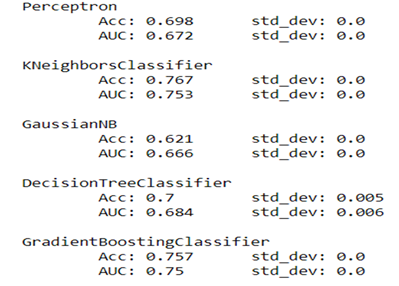
\includegraphics[width=0.6\linewidth]{figures/predictormodel1.png}
   \end{center}
      \caption{Results for Prescriber Classifier, No Cross-Validation}
   \label{fig:predictormodel1-1col}
\end{figure}

\begin{figure}[t]
   \begin{center}
      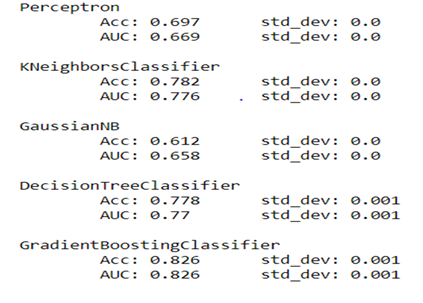
\includegraphics[width=0.6\linewidth]{figures/predictormodel2.png}
   \end{center}
      \caption{Results for Prescriber Classifier, 5-Fold Cross-Validation}
   \label{fig:predictormodel2-1col}
\end{figure}

The evaluation of our prediction models was done by splitting the data into training and testing sets. The model was also evaluated by splitting the data using stratified k-fold cross-validation.

Figure 4 shows the results we obtained on the test data for the train-test splits. According to the Train-Test Splits, the KNN and the Gradient Booster classifiers have better Accuracy and AUROC scores when compared to the other classifiers.

Figure 5 shows the results when using 5-fold cross validation. According to the 5-Fold Cross Validation, the Gradient Boosting classifier has better Accuracy and AUROC scores when compared to the other classifiers.

Looking at the average scores from the two model evaluators, we can conclude that the KNN and Gradient Booster Classifiers perform the best on the given data since they yield the highest accuracy and AUROC scores when evaluated using the train-test split and k-folds cross-validation methods.
The difference is statistically significant since the classifiers have been evaluated 100 times and the accuracy and the AUROC scores have been averaged across the 100 iterations. We can also see that the standard deviation of the scores for each classifier are very small.

From the aforementioned accuracy scores, we can see the perceptron and the Gaussian Naïve Bayes performed the worst, only achieving accuracy scores 70 and 61 respectively. An explanation to why the Gaussian Naïve Bayes performed the worst is that the GNB algorithm assumes the features to be independent of each other and for our prediction algorithm, we considered features such as credentials, specialty and list of drugs which are highly correlated. One of the reasons the perceptron performed badly is because our data was not linearly separable. The perceptron works best when the data is linearly-separable.


\subsection{State-Specific Analysis}

%-------------------------------------------------
\section{Conclusions}
%-------------------------------------------------

Overall, the goal of this project was not necessarily to find a “silver bullet” when it came to stopping the opioid crisis; indeed, if anything our analysis underscores that this issue, even when investigating just a subset of its architecture, is both complex and multifaceted. However, we feel as though we have taken a good first step into studying a piece of this crisis that hasn't already been extensively researched by other academics, at least to our knowledge. 

Our findings have allowed us to challenge conventional logic; for example, that pro-opioid lobbying would have a significant impact on opioid prescriber rates. This can of course be due to a myriad of factors - for example, perhaps this is in part due to the “bad press” around opioids and patients specifically requesting opioid alternatives - but it at least gives insight into where current funding should be focused in order to combat this crisis. We were also able to successfully create a classifier using Gradient Boosting which can perhaps be used as a starting point to identify potential “bad actors” when it comes to clinicians and opioid distribution. While we acknowledge that a large part of this crisis revolves around users overdosing from spiked or black-market opioids, many of these users get initially addicted because of opioids prescribed legally. Having a classifier which can successfully predict which doctors, based on features from national datasets, are “likely” to prescribe opioids can raise alarm when outliers arise. Finally, our local analysis using Connecticut data allowed us to pinpoint features that are prevalent in locations where opioids are commonly prescribed.

For future analyses, we think there is tremendous potential for domain-level experts to provide more insight into the raw data we utilized to perhaps garner additional insights we may have missed. Additionally, we think that our work could benefit from the addition of data we did not use or have access to, such as private datasets from drug companies. Finally, we would be interested to see future works of other states besides Connecticut to see if our findings can be replicated in different geographies. 

%-------------------------------------------------
\section{Acknowledgements}
%-------------------------------------------------

We would like to acknowledge the assistance of our Machine Learning professor, Aanchan Mohan, for his insight in the early stages of our project. He was especially helpful to us when trying to hone in on specific aspects to focus on for our analysis of the opioid crisis, taking time to help find previous scholarly works as inspiration for our final product.

%-------------------------------------------------
\section{Contributions}
%-------------------------------------------------

Overall, the amount of work necessary for this project, and its broad scope, made having four group members an asset, and allowed us to evenly split the workload relatively easily. In the work leading up to the proposal, each group member equally researched potential ideas for our project; and when we settled on the opioid crisis, we all spent time looking up datasets we could potentially use. When it came to actually writing the proposal itself, that too was more or less split equally; each of us was responsible for at least one section, and we came together to transform our prose into an acceptable LaTex format. Once the proposal was submitted and we received feedback, we also met regularly to discuss changes to our implementation and next steps.

When it came to the main piece of our project, we decided to ultimately do three unique analyses, so three of our group members took responsibility for those specific analyses. Yoselyn focused on the piece of our analysis which covered the effect of lobbying groups on opioid distribution rates; Adithya was responsible for the prescriber classifier portion of our analysis; and Matthew finished the piece on our state-level analysis. To get their analyses to work, all three of these group members needed to clean the raw datasets to their liking, and in some cases find additional datasets to complement the shared federal ones in our Github repo. They all also completed a python workbook with their findings, wrote the sections of this paper specific to their analyses, and added some slides to our PowerPoint presentation about their findings. This left Megan to handle most of the other work necessary for this project. She set up the initial Github repo holding our shared works and populated with raw datasets; helped other group members with cleaning and formatting datasets; put together the majority of the PowerPoint presentation; and wrote about half of this report, including putting it together in LaTex format.

{\small
\bibliographystyle{ieee}
\bibliography{bibliography.bib}
}

\end{document}